\chapter{Marco practico}
\label{sec:practico}
\section{Esquema General del Proyecto}
Una de las maneras más sencillas de expresar información es la gráfica. Esta sección contiene un elemento gráfico conocido como “esquema general del proyecto”, que permite observar la “arquitectura” o la forma en la cual la solución se estructura funcionalmente. Considerando que un sistema es compuesto por distintos elementos, los cuales interactúan entre sí para un fin, el esquema general tiene el propósito de presentar las relaciones entre dichos elementos.

El diagrama debe presentar los elementos del sistema como bloques. Los nombres de los elementos se incluyen dentro el bloque y se prioriza la presentación estética puesto que es imperante reconocer cada bloque por el nombre. Por otro lado, la relación entre bloques debe indicar el flujo de información, unidireccional o bidireccional, mediante el sentido de flechas incluidas en la línea de conexión. Es posible adicionar información sobre el tipo de conexión agregando algún texto sobre dicha línea. 

El diagrama debe ser elaborado mediante algún programa que permita la creación de imágenes de alta calidad, e.g. Inkscape, GIMP, Adobe Illustrator o similares. [\cite{lynch2005where}] En caso de LaTeX se recomienda el formato EPS, en cambio, para Microsoft Word es altamente sugerible emplear EMF. Si no fuera posible desarrollar tal, es necesario utilizar imágenes vectorizadas, cuya resolución sea de 300 dpi (dots per inch); se recomienda el formato PNG.

El esquema general debe ser elaborado considerando como objetivo la legibilidad y comprensión. Por tanto, el nivel de abstracción de los elementos listados en el diagrama debe ser el mismo. Cabe recalcar, sin embargo, que la prioridad radica en la funcionalidad, más no en cada componente físico del sistema; esto significa que se deben tomar en cuenta las tareas que los componentes cumplen y no a los componentes per sé.

Los componentes dentro el diagrama hacen referencia a ciertas etapas, e.g. en el caso de un sistema de visión artificial, una de las etapas será adquisición de imágenes. Estas etapas son descritas en subsecciones listadas después del esquema general. [\cite{bratkova2008metody}]

\section{Etapa 1}
Se asume que el sistema a ser propuesto es conformado por múltiples subsistemas, los cuales se ven reflejados de manera intrínseca en las etapas. Estos subsistemas tienen como objetivo abordar una parte del problema o coadyuvar a otros subsistemas a hacerlo. En el ejemplo de visión artificial, la adquisición por sí misma no puede ser definida como subproblema, no obstante, coadyuva a otras etapas o subsistemas a abordar los subproblemas. [\cite{borgman2003from}] 

Una etapa posee ciertos pasos y lineamientos que la caracterizan y delimitan el cómo debe ser realizado el diseño del subsistema respectivo. Los pasos, que corresponden a dos perspectivas: la industrial y la académica, son en general aquellos procedimientos efectuados para llegar a diseñar el subsistema. Los lineamientos se refieren a los requerimientos que definen los aspectos que deben ser tomados en cuenta al momento de desarrollar la solución. Lo anteriormente dicho refleja una verdad innegable, el marco práctico responde de forma directa al problema planteado en el marco referencial. [\cite{greenberg1998camel}]

\subsection{Requerimientos}
\subsection{Cálculos y Dimensionamiento}
\subsection{Desarrollo}
En contraparte, esta sección es adecuada para estudiantes cuyo énfasis sea el académico. Similar a lo que es requerido en “Cálculos y Dimensionamiento”, el subtítulo contiene los pasos para diseñar el subsistema especificado en el título. La única diferencia es clara, los requerimientos serán distintos para cada perspectiva; distintos en enfoque.
Las ecuaciones por desarrollar deben ser centradas.
\begin{equation}
	F = ma
\end{equation}
Las ecuaciones deben incluir el número de capítulo correspondiente y continuar la numeración en caso de no haber sido enunciadas previamente. Por ejemplo, si se enuncia una nueva ecuación ésta será insertada de la siguiente forma:

\begin{equation}
	x_1 = x_2 + x_3
\end{equation}

on ecuaciones que ya fueron enunciadas, es posible citarlas en texto: la Ecuación (3.2) es utilizada para calcular la cantidad combinada de dos elementos.

Las figuras deben tener la forma presentada por la Figura 3.1. En esta muestra un índice que permite la numeración de las figuras, la descripción de la figura que no excede de quince palabras; la extensión puede ser mayor si existen subfiguras. En casos específicos, cuando la imagen no es producida por el autor, se referencia la fuente. Si la figura fue elaborada por el autor se deberá incluir la frase “Elaboración propia”. Nótese que el tamaño de fuente es de 10 puntos.

\begin{figure}
	\centering
	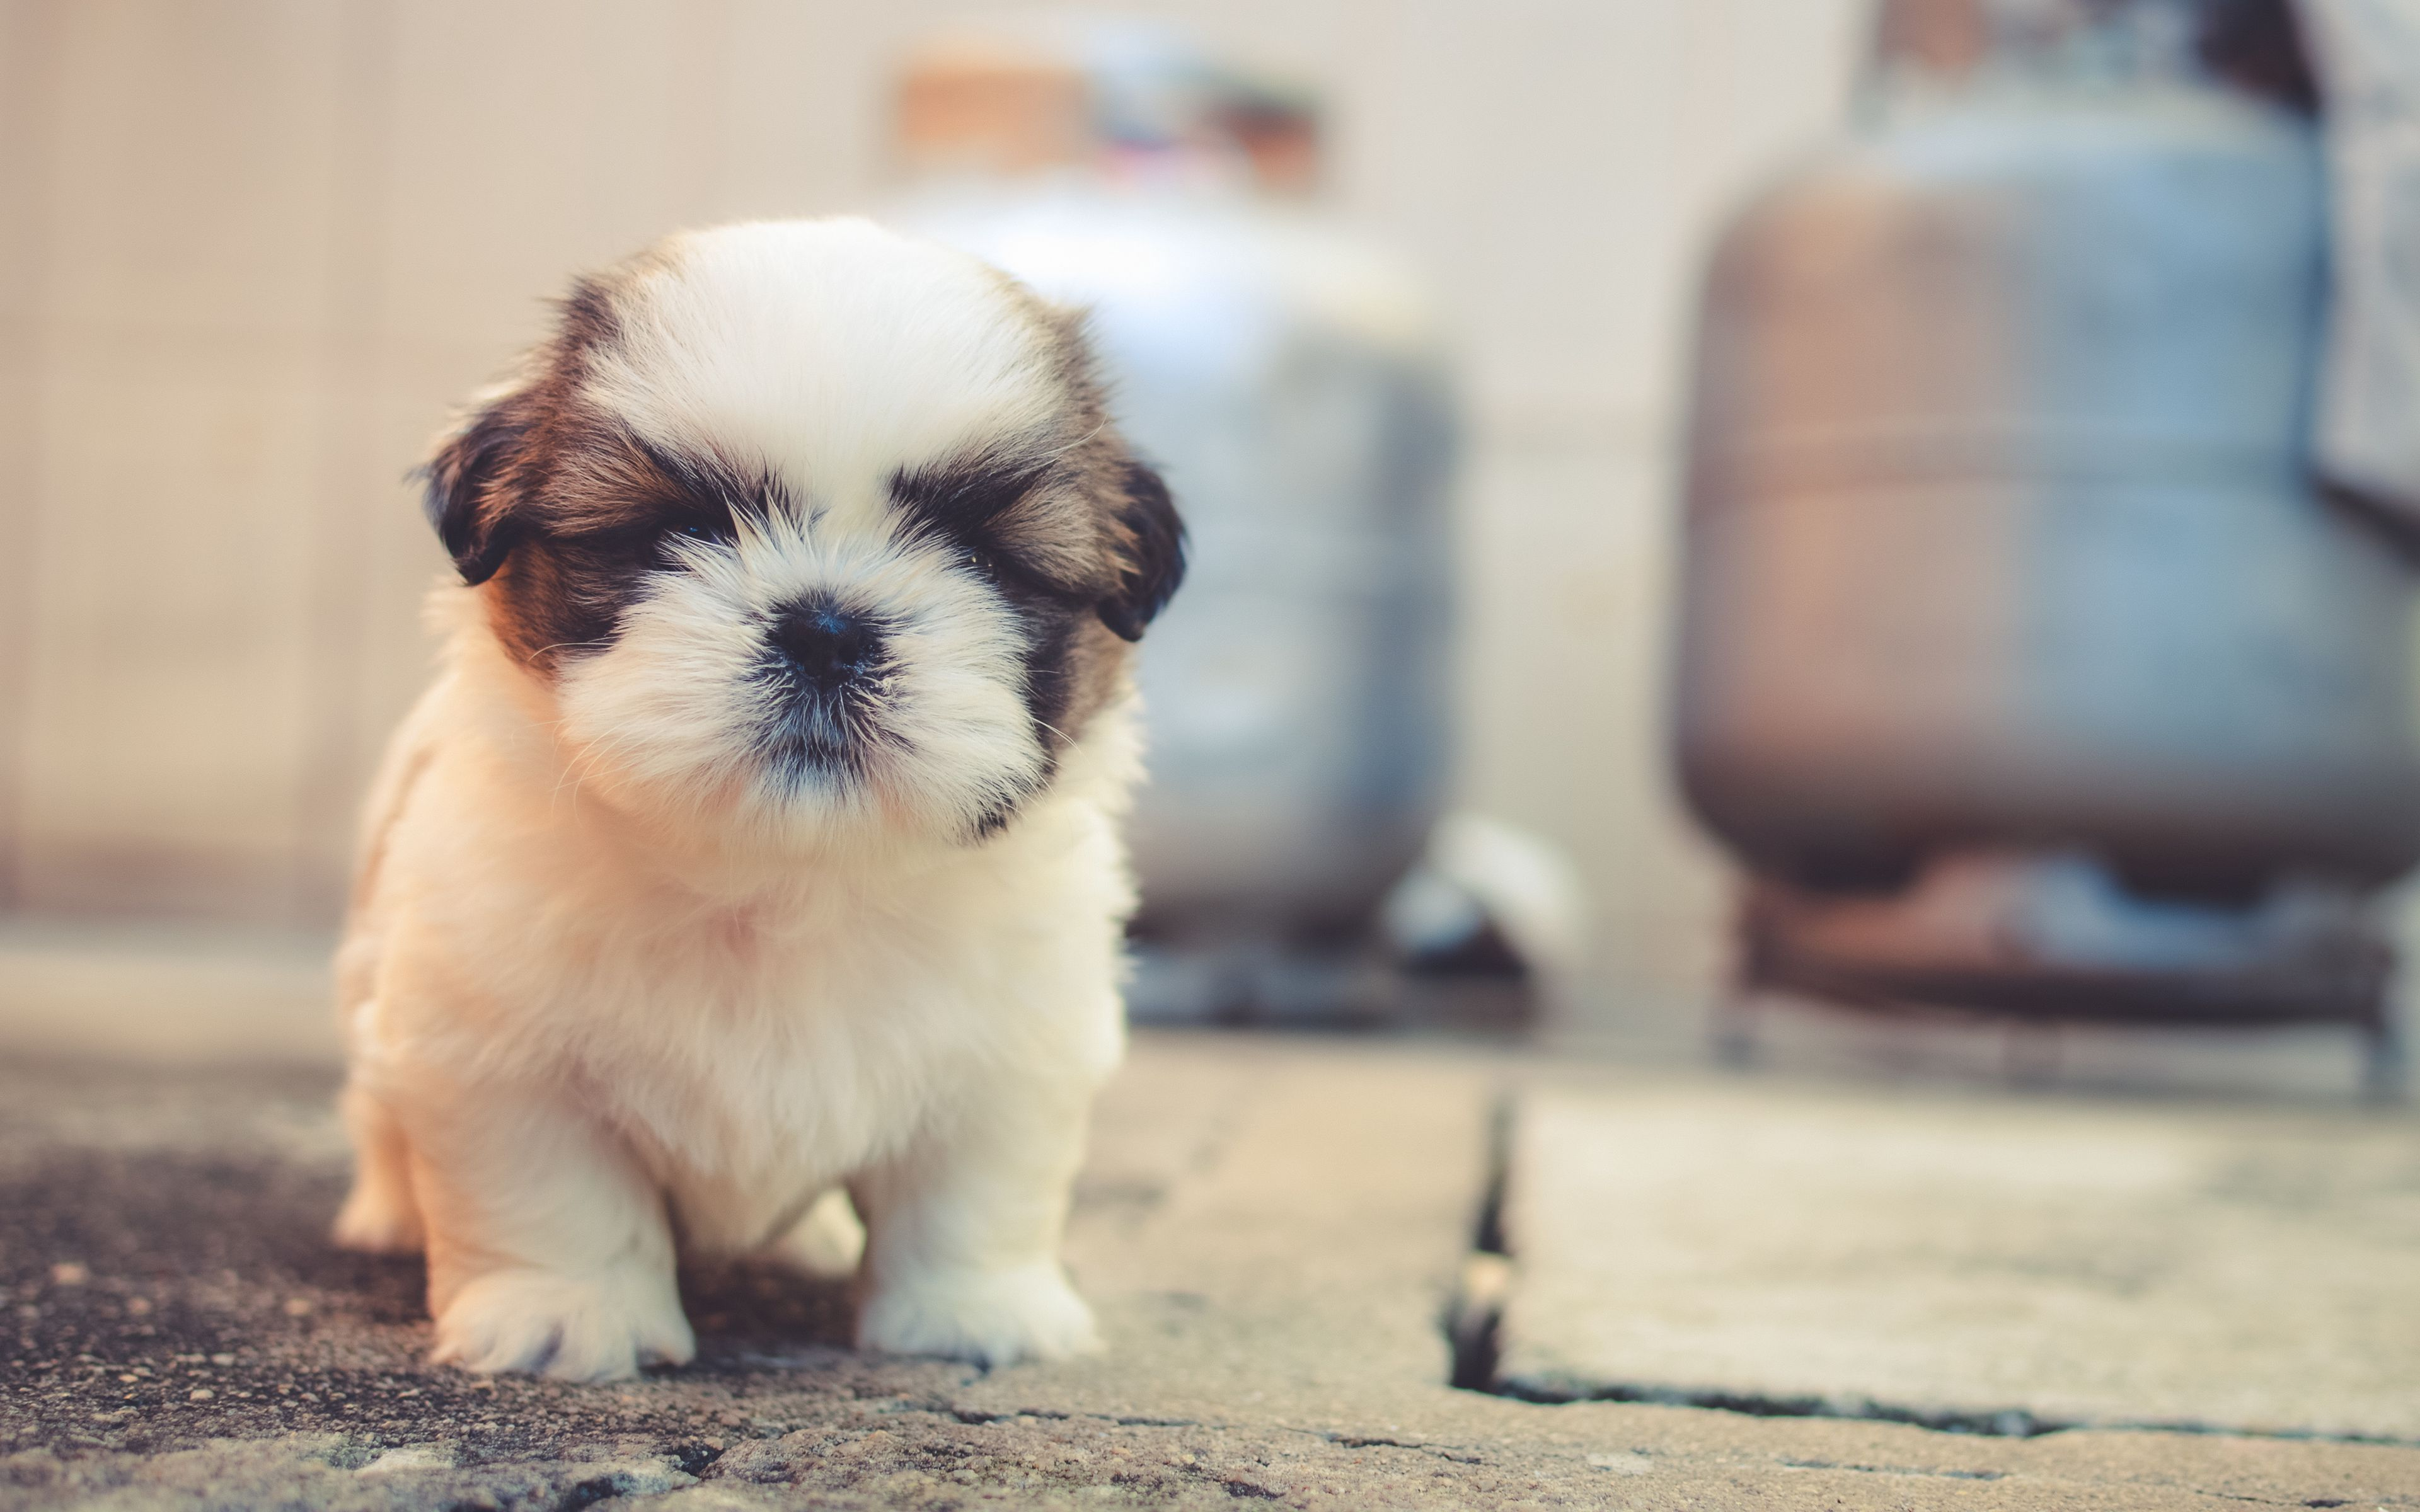
\includegraphics[width=0.65\textwidth]{images/puppy_dog_cute.jpg}
	\caption{Cute puppy} \vspace{-0.2cm}
	\footnotesize{\textbf{Fuente:} Incluir fuente bibliográfica.}
	\label{pics:Puppy} 
\end{figure}


Las figuras deben tener la forma presentada por la Figura 3.1. En esta muestra un índice que permite la numeración de las figuras, la descripción de la figura que no excede de quince palabras; la extensión puede ser mayor si existen subfiguras. En casos específicos, cuando la imagen no es producida por el autor, se referencia la fuente. Si la figura fue elaborada por el autor se deberá incluir la frase “Elaboración propia”. Nótese que el tamaño de fuente es de 10 puntos.
\begin{figure}
	\begin{minipage}[t]{0.48\textwidth}
		\includegraphics[width = \textwidth]{images/hist.pdf}
	\end{minipage}
	\hfill
	\begin{minipage}[t]{0.48\textwidth}
		\includegraphics[width = \textwidth]{images/bivardata.pdf}
	\end{minipage}
	\caption{Multiple imagenes}
	\centering \vspace{-0.2cm}
	\footnotesize{\textbf{Fuente:} Incluir fuente bibliográfica.}
	\label{pics:data}
\end{figure}

Las tablas deben disponer de líneas horizontales que delimitan el inicio, la cabecera y el final de la tabla, tal como se observa en el ejemplo de la Tabla 2.1. Cada línea horizontal tiene 1 punto de espesor. La cabecera de la tabla deberá estar en negrita y el espaciado entre líneas de la tabla deberá ser sencillo, a diferencia del espaciado en el texto normal del cuerpo de la tesis/proyecto de grado que es de 1,5 líneas. Ni la cabecera, ni el cuerpo de la tabla deberán poseer sombreado alguno.

\begin{table}[h]
	\begin{center}
		\caption{Características de desempeño SJA01 con diferentes gobernadores.}
		\label{tab:tabla1}
		\begin{tabular}{c c c}
			\hline
			           & \textbf{Tiempo de Establecimiento} & \textbf{Sobre oscilación} \\ \hline
			PID-LQR    & 17.5 [s] & 15\%  \\
			PID Kundur & 87.7 [s] & 49.08\% \\
			Mecánico-Hidráulico & 122,4 [s] & 11.1\%  \\
			\hline
		\end{tabular}\\[0.5cm]
		\footnotesize{\textbf{Fuente:} Adaptado de Viscarra (2019)}
	\end{center}
\end{table}
